\documentclass{sigchi}

% Use this section to set the ACM copyright statement (e.g. for
% preprints).  Consult the conference website for the camera-ready
% copyright statement.


% Load basic packages
\usepackage{balance}       % to better equalize the last page
\usepackage{graphics}      % for EPS, load graphicx instead 
\usepackage[T1]{fontenc}   % for umlauts and other diaeresis
\usepackage{txfonts}
\usepackage{mathptmx}
\usepackage[pdflang={en-US},pdftex]{hyperref}
\usepackage{color}
\usepackage{booktabs}
\usepackage{textcomp}

% Some optional stuff you might like/need.
\usepackage{microtype}        % Improved Tracking and Kerning
% \usepackage[all]{hypcap}    % Fixes bug in hyperref caption linking
\usepackage{ccicons}          % Cite your images correctly!
% \usepackage[utf8]{inputenc} % for a UTF8 editor only

\usepackage{todonotes}

% Paper metadata (use plain text, for PDF inclusion and later
% re-using, if desired).  Use \emtpyauthor when submitting for review
% so you remain anonymous.
\def\plaintitle{Rotakka - A Reliable \& Distributed Rotating Proxy}
\def\plainauthor{Mirko Krause, Marvin Thiele}
\def\emptyauthor{}
\def\plainkeywords{Distributed Computing; Reliable Computing; Social Media Crawling; Rotating Proxy; Big Data; Selenium; Akka; Twitter; Graph Store; Sharding }
\def\plaingeneralterms{Documentation, Standardization}

% llt: Define a global style for URLs, rather that the default one
\makeatletter
\def\url@leostyle{%
  \@ifundefined{selectfont}{
    \def\UrlFont{\sf}
  }{
    \def\UrlFont{\small\bf\ttfamily}
  }}
\makeatother
\urlstyle{leo}

% To make various LaTeX processors do the right thing with page size.
\def\pprw{8.5in}
\def\pprh{11in}
\special{papersize=\pprw,\pprh}
\setlength{\paperwidth}{\pprw}
\setlength{\paperheight}{\pprh}
\setlength{\pdfpagewidth}{\pprw}
\setlength{\pdfpageheight}{\pprh}

% Make sure hyperref comes last of your loaded packages, to give it a
% fighting chance of not being over-written, since its job is to
% redefine many LaTeX commands.
\definecolor{linkColor}{RGB}{6,125,233}
\hypersetup{%
  pdftitle={\plaintitle},
% Use \plainauthor for final version.
%  pdfauthor={\plainauthor},
  pdfauthor={\emptyauthor},
  pdfkeywords={\plainkeywords},
  pdfdisplaydoctitle=true, % For Accessibility
  bookmarksnumbered,
  pdfstartview={FitH},
  colorlinks,
  citecolor=black,
  filecolor=black,
  linkcolor=black,
  urlcolor=linkColor,
  breaklinks=true,
  hypertexnames=false
}

% create a shortcut to typeset table headings
% \newcommand\tabhead[1]{\small\textbf{#1}}

\pagenumbering{arabic}

% End of preamble. Here it comes the document.
\begin{document}

\title{\plaintitle}

\numberofauthors{2}
\author{%
  \alignauthor{Mirko Krause\\
    \affaddr{Hasso-Plattner-Institute}\\
    \affaddr{Potsdam, Germany}\\
    \email{mirko.krause@student.hpi.de}}\\
  \alignauthor{Marvin Thiele\\
    \affaddr{Hasso-Plattner-Institute}\\
    \affaddr{Potsdam, Germany}\\
    \email{marvin.thiele@student.hpi.de}}\\
}

\maketitle

\begin{abstract}
  In today's data-driven world, a lot of research is dependent on the availability of data. Social networks own vast amounts of interesting data and the analytical possibilities could range from simple statistics to complex text mining. Unfortunately, the data is often either not available or not affordable. Therefore, it is interesting to collect at least the data that has been made public. We chose to build a system capable of downloading such public data at scale. Our sample use case tackles tweets on Twitter.
  
  We propose Rotakka, a distributed cluster application designed for scalable Twitter crawling. Its main advantage is that it avoids IP-based blocking by exploiting publicly available web proxies. In contrast to API-based approaches, Rotakka uses browser emulation enabled by Selenium to visit and download Twitter user profiles. It is built on the Akka framework and consists of a proxy-collecting module, a proxy-checking module, a Twitter-crawling module, and a graph-storing module. 
  
  The addresses of the proxy servers, which are used by the Selenium browsers to hide their real IP address, are gathered from public proxy repositories. In order to use only working proxies for the crawling, all proxy addresses must pass an availability check. All information gathered by the Twitter-crawling module is converted into subgraphs consisting of vertices and edges and passed to the graph store. There the graph elements are assigned to shards, which are stored replicated on different servers.
  
\end{abstract}

% ACM Classfication

\begin{CCSXML}
<ccs2012>
<concept>
<concept_id>10010520.10010575</concept_id>
<concept_desc>Computer systems organization~Dependable and fault-tolerant systems and networks</concept_desc>
<concept_significance>500</concept_significance>
</concept>
<concept>
<concept_id>10010520.10010575.10010577</concept_id>
<concept_desc>Computer systems organization~Reliability</concept_desc>
<concept_significance>300</concept_significance>
</concept>
<concept>
<concept_id>10002951.10003260.10003261.10003263.10003262</concept_id>
<concept_desc>Information systems~Web crawling</concept_desc>
<concept_significance>300</concept_significance>
</concept>
<concept>
<concept_id>10010520.10010575</concept_id>
<concept_desc>Computer systems organization~Dependable and fault-tolerant systems and networks</concept_desc>
<concept_significance>500</concept_significance>
</concept>
<concept>
<concept_id>10010520.10010575.10010577</concept_id>
<concept_desc>Computer systems organization~Reliability</concept_desc>
<concept_significance>300</concept_significance>
</concept>
</ccs2012>
\end{CCSXML}

\ccsdesc[500]{Computer systems organization~Dependable and fault-tolerant systems and networks}
\ccsdesc[300]{Computer systems organization~Reliability}
\ccsdesc[300]{Information systems~Web crawling}


% Author Keywords
\keywords{\plainkeywords}

% Print the classficiation codes
\printccsdesc


\section{Introduction}

In today's world of Big Data, social media platforms, such as Twitter or Facebook, hoard tremendous amounts of data. While the majority of this information is displayed to the public, it is very hard to gain a comprehensive overview of everything happening in these networks. Researchers around the world are strongly interested in this data in order to evaluate the social structure on these networks or train cutting edge machine learning models. % TODO: REFERENCES wenn zeit

To grant access to the data, some platforms like Twitter offer several levels of API access. However, most offers either do not scale up to the wished volume of data, or are just too expensive for the average researcher. 
At this point, many researchers choose to circumvent the API limitations by crawling the data in an automated fashion directly from the website. Aware of this fact, social media platforms often enforce counter-measures such as IP- and account-blocking to harden themselves against this form of data extraction.

As a solution for these problems, we propose \textbf{Rotakka}, a distributed and reliable rotating proxy with an integrated social media crawling use case featuring a basic graph store.

Compared to a more basic, monolithic, and local approach, Rotakka has multiple advantages: Firstly, it is designed for a distributed setting. It can take advantage of multiple Internet connections and exploit a large resource pool. Secondly, it avoids IP-based blocking by continuously changing the outfacing IP address in a rotating manner, thus effectively mimicking a rotating proxy. In order to distribute the outgoing connections, public proxies are being used. The required proxy servers are being gathered from external sites offering free proxies and tested by the responsible modules of the Rotakka system.

Rotakka is built with \textbf{Akka}, a "toolkit for building highly concurrent, distributed, and resilient message-driven applications for Java and Scala" \cite{akka:homepage}. Akka implements the actor model, which is highly useful for building distributed applications. In a nutshell, every semantic component of a system becomes a separate entity, called an actor. Actors have their own private state and communicate with other actors by sending mostly asynchronous messages to them. These messages may contain arbitrary information (generic serializable Java 'Objects') triggering the wanted behavior and often leading to the creation of new messages. This encapsulation of computation allows a highly concurrent, in the best case even non-blocking control flow.

\section{Related Work}
\label{sec:related_work}

For our crawling tasks we use \textbf{Selenium}, a "suite of tools to automate web browsers across many platforms" \cite{selenium:homepage}. Currently, it supports at least Firefox, Chrome, and Chromium on the most common operating platforms, namely Windows, MacOS, and Linux. For our use case, the toolkit allows us to visit websites similar to a human user, meaning JavaScript gets executed and all images are loaded. This costly procedure results not only in the benefit of us being more stealthy, it also ensures a proper website-server as well as website-user interaction on JavaScript-enabled pages. In addition, we can even have a real-time look at the websites our code is visiting. However, the most important factor hereby is still the JavaScript execution, because it enables data extraction out of dynamically loaded content. Other software typically used for crawling content, such as JSoup \cite{jsoup:homepage} or Crawler4j \cite{crawler4j:github}, are static HTML parsers. They lack the JavaScript execution and, therefore, are not suited for dynamic websites. A considerable alternative to Selenium could have been PhantomJS, but its development has been put on hold \cite{phantomjs:homepage}, so we decided not to use it.

The downside of using browser automation tools such as Selenium are the high resource requirements, namely RAM and CPU. However, given that Rotakka is a distributed system, it can use, in theory, an infinite amount of RAM and CPU through scaling. Also, scaling out to more machines is usually cheaper than scaling a single machine up to an equivalent performance.

Acknowledging the previous arguments, the popularity, and the professionalism of Selenium, we decided to integrate it into Rotakka.

However, Rotakka is not the only player on the market. There are systems that aim for the same goal. The main difference between Rotakka and its rivals is that the other systems exploit the free-tier of the official API and circumvent the request limitation by using many different IP-addresses. These, however, cannot all be blocked. In order to achieve this, Noordhuis et al. have for example used the AWS cloud for their Twitter Cloud Mining \cite{twitterCloudMining}. Bo\v{s}njak et al. followed a similar approach but were using other, unspecified clouds for their TwitterEcho \cite{twitterEcho}.


\section{Architecture Overview}

As seen in \autoref{fig:abstract_arch}, Rotakka can be split into three distinct subsystems: 

The first subsystem is the proxy crawling and checking system (PCC). It is responsible for continuously crawling new public proxies from public proxy lists and periodically checking the performance of already gathered proxies. 

The resulting proxies are then needed by the Twitter crawling system (TC) that will send proxied web requests to the Twitter servers. The proxies maintain a changing set of outfacing IP addresses during the Twitter website requests. Furthermore, the TC controls the connection between the browsers (running Twitter websites) and the Twitter servers, while extracting the relevant information from the website.

The last subsystem is the Graph Building and Storage system (GBS). Its main task is to safely persist the data gathered by the TC by integrating it into a distributed graph structure.

\begin{figure}[h]
\centering
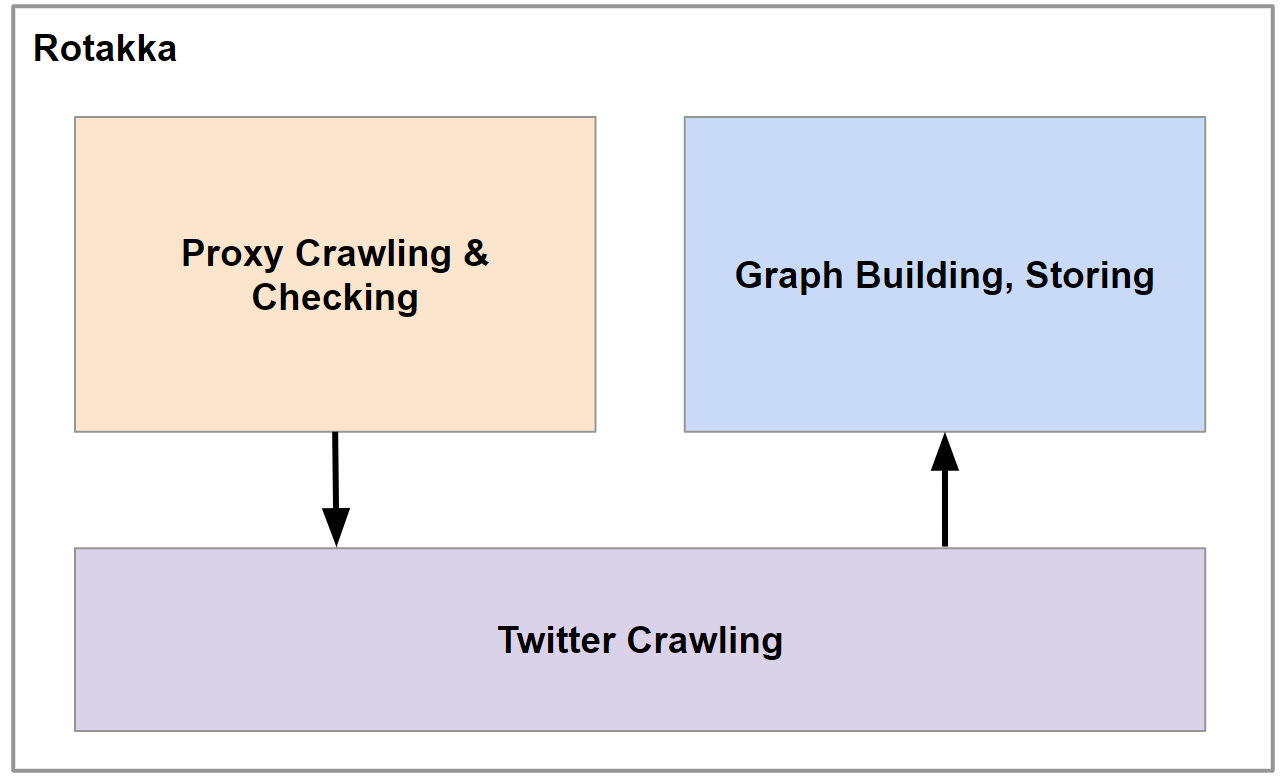
\includegraphics[width=8cm,height=8cm,keepaspectratio]{figures/abstract_architecture.PNG}
\caption{Abstract Architecture of Rotakka}
\label{fig:abstract_arch}
\end{figure}

Having the general structure in mind, we now want to dive deeper into the more specific architecture of each subsystem, where we will have a look at the responsible actors and their interactions. The in-depth structure of Rotakka can be seen in \autoref{fig:detailed_arch}. Every block represents a specific kind of actor within the system. Cluster singletons are  marked by a thick black border. Those exist only once in the whole cluster. If one system that hosted a cluster singleton goes down, the Akka-internal singleton managers will agree on an online system on which they restart the singleton instance.
In contrast to the singletons, all other actors exist more often, there is usually at least one per system. How many actors there really are created on each system depends on the run-time configuration and the run-time needs. For instance, there may be one GraphStoreSlave per system, but there can be many GraphStoreBuffers on the same system as the GraphStoreMaster. For now, it is important to note that the number of actor instances of every actor kind is not further illustrated in \autoref{fig:detailed_arch}. More information on this step will be given in later sections. 

A constant design pattern across Rotakka is the Scheduler-Worker pattern, which is better known as the Master-Slave pattern. The scheduler is responsible for coordinating and spreading tasks across multiple workers. For example, the ProxyCheckingScheduler collects all the proxy addresses crawled by the ProxyCrawlers, and distributes the task of checking the addresses across the ProxyCheckers. The other schedulers work by a similar pattern (ProxyCrawlingScheduler and TwitterCrawlingScheduler).

Mapping the PCC-system to \autoref{fig:detailed_arch}, we can see by the prefixes that it is further split into two parts: the proxy crawling and the proxy checking. 
Each part consists of one scheduler and multiple workers. The TC-system is split in the same way. 

In contrast, the GBS-system has a slightly different structure. It has no scheduler and there is no work to be distributed. 
Instead, the GraphStoreMaster receives graph elements and forwards them to the responsible GraphStoreBuffers. These buffers either buffer the graph elements or forward them to the GraphStoreSlaves, where the vertices and edges are stored. In summary, the GraphStoreMaster is responsible for distributing the data and keeping a consistent state.

Furthermore, in \autoref{fig:detailed_arch} we see another actor that was not mentioned yet, the DataReplicator. This actor is responsible for resiliently saving data and will be explained in detail in \autoref{sec:data_replicator}.

\begin{figure}[h]
\centering
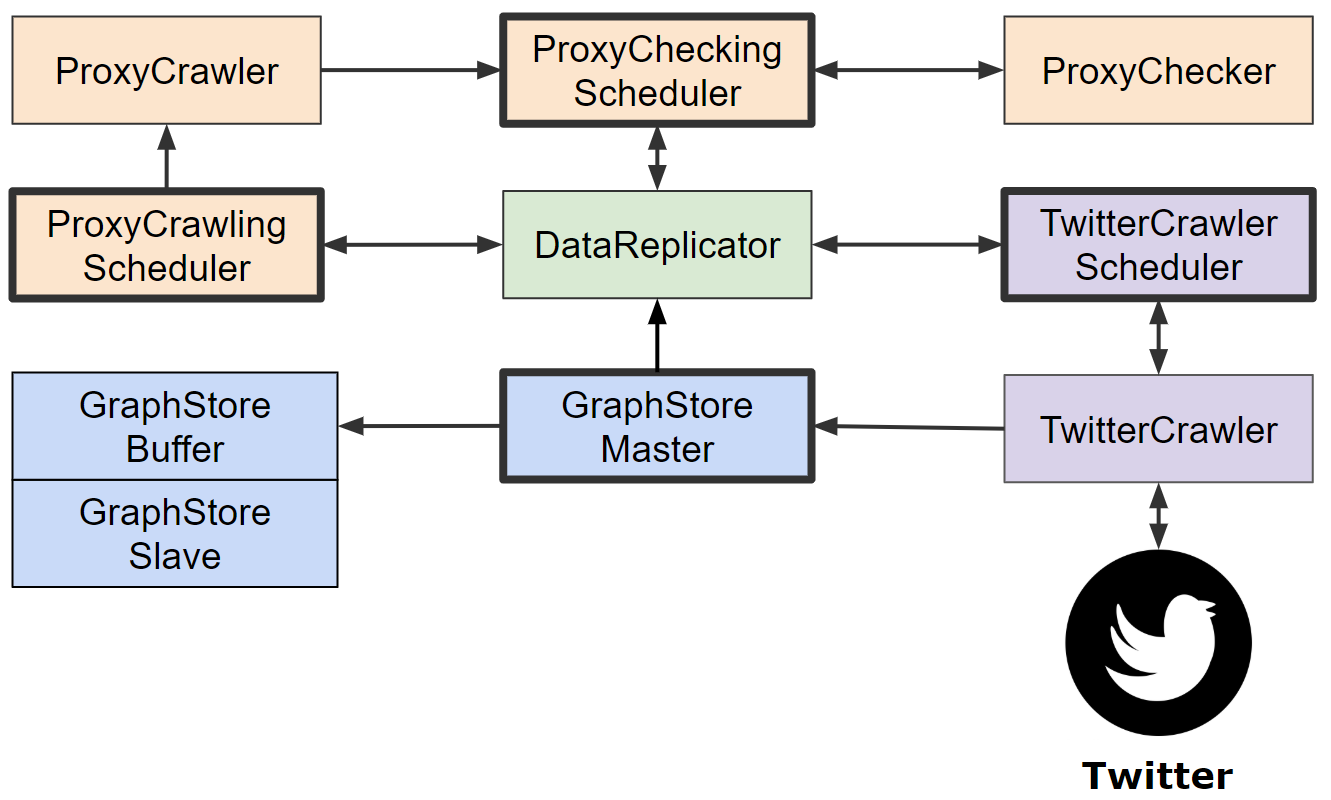
\includegraphics[width=8cm,height=8cm,keepaspectratio]{figures/detailed_architecture.PNG}
\caption{Detailed Architecture of Rotakka}
\label{fig:detailed_arch}
\end{figure}


\section{Public Proxy Crawling}

An abundance of public proxies can be found on the Internet. However, only a minority of these free proxies is useful. Research shows that only 38.23\% of public proxies are reachable and properly forwarding the traffic \cite{fast_dist_crawling}, which makes availability checking essential in order to be able to use the proxies. Furthermore, the same paper mentions that after only two days, only 81.62\% of the initially working proxies are still available. This increases the importance of constantly checking whether proxies are (still) alive or not.

To prevent port-scanning the whole Internet for proxies, we crawl our proxy addresses from multiple, publicly available websites. Unfortunately, some of the proxy pools do not favor being crawled, because competitors can gain an advantage by enlarging their own proxy lists.  During our work, we have discovered interesting ways of how these websites defend themselves against automated extraction of their data. The countermeasures ranged from base64-encoded data to instant IP-blocking as soon as automated crawling is detected. However, by using browser emulation and restrained crawling, we are able to surpass these countermeasures. The information we finally extracted from these websites are the IP addresses, the TCP ports, and the proxy types.

There are multiple types of proxies. The most common types are HTTP, HTTPS and SOCKS proxies. Only the HTTPS and SOCKS proxies are valuable for our use case however, given that Twitter is only reachable via HTTPS.

In order to check a proxy, we have to go through several steps:
Firstly, we determine whether the proxy server is reachable. This reachability check is a functionality from the Java standard library, typically implemented by using an ICMP echo request (ping). 
Secondly, we try reaching Twitter by using this proxy. If both steps are successful, then, thirdly, we estimate the average response time of the proxy by measuring the time needed in order to connect to \url{google.com}. Furthermore, we only take fast proxies into consideration which examine a response time below a configurable limit (around 300ms). This prohibits the system from using very slow proxy servers, which would obstruct the overall crawling process.

To better understand the flow of actions within the PCC-system, we want to present the different actions the subsystem takes. Inherently, the ProxyCrawlingScheduler knows different sites that offer public proxies. Because each of the known websites is unique, we had to write code to adapt to each of them. The ProxyCrawlingScheduler then creates work packets and distributes the actual crawling jobs to different ProxyCrawler actors. The scheduler knows its workers, because they sent it a registration message during their startup process. This registration is part of every scheduler-worker as well as every master-slave relationship. After the work packets have been distributed, the ProxyCrawlingScheduler will continue by scheduling a recrawling of the proxy websites to stay up to date. 

Having received a work packet, the ProxyCrawler actors start to extract the proxy addresses from the given website and send them to the ProxyCheckingScheduler. This scheduler puts the received unchecked proxies into a work queue and assigns them to the ProxyChecker actors in a pulling manner.
When a ProxyChecker receives a work packet, it checks the proxies and sends their status back to the ProxyCheckingScheduler. Those proxies that passed the test will be persisted in the DataReplicator. The non-working proxies will be discarded and eventually be rechecked, caused by a scheduled recrawling of the proxy list websites.

\section{Social Media Crawling on Twitter}

The Social Media Crawling implemented in Rotakka is strongly adapted to Twitter, which is our main use-case. The entry points of our system into Twitter are one or more usernames. The tweets of these specific users will be crawled first. All other accounts that are found in the crawled tweets are then consecutively crawled as well. This is the case when the originally crawled user has retweeted or mentioned another user. It is also possible to disable this branching behavior if only the specified users should be crawled. In addition to the initial user profiles, Rotakka also needs a tweet-limiting time frame. In order to crawl tweets and to set a time frame, we use Twitter's advanced search functionality, which allows us to see all tweets posted in a certain time period. However, if the time frame is too generous, not all tweets will be shown. This is a limitation implemented by Twitter. To circumvent this problem, we initially decided to crawl the tweets in monthly intervals, which was usually enough to get all tweets from a user within that time frame. After a big update of Twitter in July 2019 \cite{twitter:update}, the results from the advanced search dropped from around 500 to a range between 50 and 170, depending on the account. This made us reduce the crawling time-interval to one day in order to maintain data completeness, which is one of our main goals. However, this lead to a significant drop of tweets per second (TPS) in Rotakka.

As mentioned before in \autoref{sec:related_work} however, the website crawling itself is done by Selenium. 

The control flow of the TC subsystem happens as follows: Firstly, the TwitterCrawlingScheduler generates work package from the initially configured usernames. A work package is a link to Twitter's Advanced Search and contains a user and time frame. These work packages are then sent to the many TwitterCrawler actors, which will extract all tweets and send the information to the GraphStoreMaster. Moreover, any user that has been found will be sent to the TwitterCrawlingScheduler for further processing.

Furthermore, each TwitterCrawler has access to exactly one Selenium instance. Instead of implementing the proxy as a separate part of the system, we decided to integrate the different proxies directly into the browser. Since the proxy addresses are immutable within the Selenium instances, the TwitterCrawlers also manage the intervals at which they restart their Selenium instance in order to change their used proxy. Therefore, after a number of work packages, the browser will be restarted with a different proxy to avoid blocking.

% Latest Mode and Exact Mode

\section{Graph Building and Storing}

\subsection{Data Model}

Rotakka includes a basic distributed graph store to persist the information collected by the TwitterCrawlers. We decided in favor of a graph model for the collected data, because Twitter is a social networking platform and, therefore, represents profiles and their interactions. These are comparable to the real-life human interactions. Our graph consists of vertices (comparable to objects) and directed edges (comparable to arrows between the objects).

The graph store is capable of storing vertices and edges. Vertices consist of a necessarily unique string key and a properties dictionary mapping from strings to objects. Edges also have a unique string key and a properties map, but, in addition, they contain the key of their start and end vertex. Our graph is not made for graph analytics though, so it is not mandatory for the vertices to maintain a list of their in- and outgoing edges. Graph traversals would be anyway unfavorable from the performance point of view, because neighbor vertices are most likely not on the same server.

Ongoing research still exists on tackling the question of how to partition a graph into shards. It is beneficial to have a minimized number of edges ending in two different graph shards. This question is important for every graph database that offers graph traversals, because the locality of traversed vertices has huge impacts on the traversal performance. Every time the graph traversal leaves the shards on a server, it undergoes a decrease of speed given that the memory access is quicker and better accessible in comparison to the slower network connection. Therefore, we chose not to implement any complicated access possibilities in the graph store. Graph elements (vertices and edges) can only be created, updated and queried by their key. For our Twitter crawling use case however, no more capabilities were needed. Nevertheless, the graph store can be extended if necessary.

\subsection{Sharding and Replication}

The main goal of the graph store is to persist the graph elements it received. The second main goal is to be able to scale out. These goals are achieved by splitting up the graph into shards. Every shard should be so small that every server of the cluster is able to keep multiple shards in memory. The graph elements are assigned to the shards based on the hashcode of their keys modulo the overall number of shards. This method is called consistent hashing. However, the hashcode assignment often results in different-sized shards. This can be a problem in a cluster, if one server gets all the big shards or, even worse, only one shard gets populated. Anyway, the problem can be solved probabilistically by increasing the number of shards. An increased number of shards probably reduces the maximal size difference between two shards. Therefore, every server should keep multiple small shards, which hopefully have a similar size. As a rule of thumb we have chosen to use at least 8 shards per server.

The total number of shards must be specified when starting the GraphStoreMaster and it cannot be changed while the cluster is running. This means, that the first servers in the cluster have to keep many shards, but the shards will be handed over to servers that joined later. However, regarding the main goal of keeping the graph data safe, shards do not prevent data loss in case a server fails. Therefore, every shard is stored on multiple servers simultaneously. Usually, a duplication level of three is recommended to keep data really safe.

\subsection{Actors and their Responsibilities}

In contrast to the other subsystems, the graph store is a master-slave system, where the GraphStoreMaster is the only actor that is supposed to apply changes to the graph store. Even though a multi-master or even a leaderless system would be much faster, we have put more focus on data consistency, which is easier to achieve with a single master.

The graph store consists of the GraphStoreMaster, which is a cluster singleton, $shardCount * duplicationLevel$ many GraphStoreBuffers on the same node as the GraphStoreMaster, and $serverCount$ many GraphStoreSlaves on different servers, by default one slave per server. The GraphStoreMaster is the single entry point into the graph store. When graph elements (either a vertex, an edge, or a subgraph) arrive, the master assigns shard IDs to them and forwards them as sharded graph elements to the GraphStoreBuffers. Every buffer is responsible for exactly one shard copy (one shard contains $duplicationLevel$ many identical shard copies). The GraphStoreBuffers play an important role when a shard copy should be moved or copied. The real shard holders are the GraphStoreSlaves. Those store a map from their assigned shard numbers to their shard copies. Every shard copy consists of two maps, each mapping from the graph element keys to the belonging vertices or edges, respectively. Because of this differentiation, there can be an edge with the same key as a vertex, but vertices with the same key will have their properties merged. New properties with the same property key will override the previous property value. This merging is true for edges, too.

\subsection{Data Persistence}

In order to keep the vertices and edges even after shutting down the system, a basic append-only file storage is implemented in the slaves, called GraphFileOutput. The GraphStorageSlave will recognize if a vertex or edge already exists. A received graph element will either be created, updated or left untouched. In case a vertex is newly created or updated, it will be appended as Json to a local vertices.json file in a directory dedicated to the GraphStoreSlave and the specific shard. In such a directory is also an edges.json file, so the same states for edges. It can happen that the same graph element key appears multiple times in the graph storage file (in case the graph element has been updated). In such a case, the graph storage file includes all versions of the graph element. For further processing it is recommended to keep only the last Json object of each key to work on the latest data. There is also no guarantee that all graph element versions are kept, because sometimes it is necessary to copy or move shard copies to a different slave. In this case, only the in-memory dictionaries with the latest graph element versions are copied to the new slave. The previous versions get lost when the shard is unassigned from a slave and all shard elements are removed from this slave. Especially shard moving ends with deleting the shard copy from the initial shard holder.

We have decided to shard the graph, because it might get quite large if many servers are crawling together for a long time. This case could not be excluded. However, the disadvantage is that the graph is split into multiple files on many different servers. For graph analytics we suggest a system that is able to handle such widespread data, for example Apache Spark, possibly with the GraphX module.

\subsection{The Shard Copying Process}

Especially in the early phases of the cluster and whenever a new slave joins the cluster, the GraphStoreMaster assigns shards to slave, optionally sending an attribute about the previousShardHolder. If this attribute is not set, the master assigns the shard to the slave and the slave creates an empty shard copy in its storage. This empty attribute is the case for every first slave of each shard. If there is already at least one slave, the new slave needs to copy the shard copy from the previous shard holder. Therefore, the new GraphStoreSlave sends a shard request to the previous shard holder. The previous shard holder will then tell the GraphStoreMaster to initiate a new copy procedure, started by telling the GraphStoreBuffers for the old and new shard copy to start buffering to keep both shard copies in a consistent state during the copy procedure. 

After the buffering has been enabled, both slaves get a notification. As long as the buffering is enabled, the master can continue sending new incoming graph elements to the buffering buffers, where the graph elements get appended to local object queues. Therefore, if the copy procedure takes too long or the master receives too many new elements, the master system may run out of memory.

As soon as the previous shard holder receives the StartedBuffering notification from its GraphStoreBuffer, it starts sending the shard content as one subgraph to the new (requesting) slave, which will acknowledge the receivement. In addition, the requesting slave will notify the master of the copied shard being ready. The previous shard holder will do the same upon receiving the acknowledgement. When the master receives the ShardReady notification it tells the belonging GraphStoreBuffers to stop buffering, at least as long as there are not more than $duplicationLevel$ many shard copies available for the copied shard. If there are too many shard copies, the GraphStoreMaster instead removes the GraphStoreBuffer of the previous shard holder and tells the previous shard holder to remove its shard copy such that the number of shard copies equals the $duplicationLevel$ again.

Unfortunately, in a distributed system it is possible that multiple copy processes overlap, for example, if a new slave joins and a shard that is still in the copy process gets assigned to the new slave. The new slave requires a different state of the shard, because its clean buffer does not know the graph elements that the buffer of the previous shard holder already received during its buffering. Copying the already received graph elements from the previous buffer could have caused race conditions, for example because of inbox queues, so we decided to prevent overlapping copy procedures that work on the same shard copy. Therefore, the GraphStoreMaster also maintains a copy procedure queue for every shard copy. Incoming InitializeCopy commands may have to wait for the previous copy procedure to finish and, after a copy procedure finished, it can happen that the master tells the buffer to stop buffering and directly sends a second message to start buffering again. 

\section{Data Replicator}
\label{sec:data_replicator}

The data replicator actor is represented in Akka Distributed Data framework as the replicator. Its main function is "to share data between nodes in an Akka Cluster" \cite{akka:dddoc} by implementing a key-value store with CRDTs (Conflict Free Replicated Data Types). The main benefit of this replicator is its presence on every node of the cluster, which makes it very fault-tolerant. 

The different scheduler actors within our system hold important state which needs to be kept safe under any circumstance. For example, knowing which Twitter users have already been crawled is essential. Therefore, we use the Akka replicator, which we have named DataReplicator, to keep this state safe.

The idea behind this behavior is that in case of a node failure, or any other case in which a scheduler becomes unavailable, we can restart this specific actor on another node and recover its previous state from the DataReplicator. Therefore, we effectively eliminate the fact that masters in master-slave patterns are usually single points of failure.

While the value of the state of slave actors like a TwitterCrawler-actor is not negligible, we decided to not persist the current work of the slaves. In the grand scheme of things, a single day of tweets is not important enough to justify the use of the DataReplicator. Since every piece of data which enters the DataReplicator is repliacted to all nodes, we only perform this step for the most valuable types of data in our system. Additionally, other systems like PCC are self-healing in a way that they will re-execute a dropped crawling task after a certain time.

\section{Evaluation}

Multiple metrics come to mind when evaluating a distributed crawling system like Rotakka. The first is measuring the Tweets Per Second (TPS) across the system. The metric strongly correlates with the selection of users which are crawled, since frequently tweeting users have more Tweets per day to scrape.

A unbiased metric is the Work Packets per Second (WPS). A work package in the TC subsystem is defined as crawling a single day of Tweets from a specific user. This metric allows for a more balanced view on performance, as it is more stable in regards to the Tweet frequency of users. However, high-frequency accounts will still take longer per work-packet than low-frequency accounts.

The test cases we choose to evaluate our system at scale are reasonable small and can be finished in less than two minutes of crawling time. This size was motivated by not unnecessarily abusing the Twitter service and keeping the crawling, which is a term of service violation, limited. 

\subsection{Twitter API}

The correct way of downloading large amounts of Tweets is using the official API provided by Twitter. While the free level offers a user to download 5000 Tweets per month (50 request \'{a} 100 Tweets), the premium service goes up to 1.250.000 Tweets per month (2.500 requests \'{a} 500 Tweets) for a price of 1899\$ per month. Moreover, there is also an enterprise-grade API, but there is no public information about the details of this level. \cite{twitter:pricing}

\subsection{Single Node Test}
We evaluated Rotakka on a Windows laptop featuring a four-core Intel i5-7300HQ @ 3.50GHz processor and 16 GB of RAM. To eliminate external factors, we choose to crawl all Tweets from the high-frequency account of the British newspaper "The Guardian" in 2018. We disabled the proxy usage to single out the maximum one node performance. Moreover, we run three TwitterCrawler-instances.

This test resulted in scraping 29.402 Tweets in 15 minutes and 16 seconds, which results in 32 TPS while fully occupying the CPU for the complete time-frame and using about 2.5 GB of RAM. Since it is a high-frequency account, we only achieved a WPS of 0.4. The network usage is considerably low and peaks out at about 8 MBit/s.

When comparing single-node, low-resource Rotakka to the premium service, we can see that we could scrape the monthly limit of the highest commercially available level (1.25 Million Tweets) in about 10 hours and 51 minutes on a single machine. This result shows the strong capabilities of Rotakka in setting optimized for high TPS (i.e. no proxy, high frequency account). Effectively, running Rotakka on a single node would save a researcher about 1899\$ in API fees every 11 hours at maximum.


\subsection{Cluster Test}
To evaluate Rotakka in a distributed setting, we run our application on a cluster consisting of 12 nodes. The machines have 20 Intel(R) Xeon(R) CPU E5-2630 processors with a speed of 2.20GHz each. The available RAM differs on the specific machine, but is either 30 GB or 60 GB. However, since we do not utilize more than 30 GB of RAM, this difference is insignificant to our test. 

As our test case we choose one year of activity from eight major global news outlets including "The Guardian" and the "Wall Street Journal". Like in the single node test, we disabled the proxy usage to maximize performance. We used 16 TwitterCrawler-actors per slave node.

This test resulted in scraping 184.625 tweets in 1 minute and 44 seconds, which equates to 1775 TPS and 28 WPS. To put this result into perspective, we can look again at the maximum limit of 1.25 million Tweets from the official API. Rotakka would be able to reach this limit in about 704 seconds or in under 12 minutes. Regarding the WPS, Rotakka is able to crawl about a month of tweets from a high-tweeting user per second. These results illustrate the capabilities of our proposed system.

\subsection{Scaling Factor}
When examining distributed systems, the efficiency of scaling these systems horizontally is a crucial evaluation step. To examine this metric, we compare the TPS of two machines and 12 machines to see how close the system gets to linear scalability. The test shows that 2-node Rotakka has a performance of 309 TPS, which means that a 12 node cluster should, when Rotakka is linearly scalable, have 1854 TPS. However, we evaluated in the previous test that we can only achieve 1775 TPS, which results in Rotakka scaling at 95.74\% of the linear scalability.

We choose to run this test on two instead of one node because the performance influence of the Schedulers is higher in a one-node setup. To eliminate this bias, we chose to take two nodes as the base scenario.


\section{Future Work}

In the context of the seminar "Reliable distributed Systems Engineering" we built the Rotakka system to the best of our ability. However, there are multiple spots in the system where future work could take place in order to improve the capabilities of Rotakka.

Regarding the PCC-system, we could imagine gathering more information about the crawled proxies, such as the origin country. This could enable Rotakka to be used for crawling geolocked websites. More research regarding automatic crawling of proxy servers would also be interesting. Multiple approaches seem feasible in this direction. The proxies could either be extracted by regex from the free proxy sites, which would drastically reduce the manual coding efforts, or automatically searched and extracted via the IoT search engine Shodan \cite{shodan:homepage}.

Additionally, Rotakka could be extended in such a way that it can handle an inert external proxy list file. This could be used to give Rotakka access to predictable, high-quality proxies, which would not strongly affect efficiency. This change would also entail integrating the ability to use proxies with authentication.

Moreover, one would also need to integrate more public proxy repositories into Rotakka. The current selection of these pages is limited and can be seen as a proof-of-concept. However, when crawling at scale, Rotakka needs access to a large pool of public proxies in order to fulfil its role effectively.

The TC subsystem could also be extended by several interesting features. When deciding which user to crawl next, one could image using a priority queue sorted after the amount of followers of that specific user. This would allow the system to crawl more influential users first. While looking like an easy change, we would need to implement a separate actor which would visit the profiles of new found users and extract the follower count. 
Moreover, one could think about implementing a maximum crawling depth. This would allow Rotakka to stay close to the original user, rather than potentially deep-diving into certain parts of Twitter. 
In addition to these smaller changes, Rotakka could also be extended to work with hashtags instead of users. This shift in paradigm could offer new use cases.

A more general issue with Rotakka is configuration. A user has to estimate how many TwitterCrawler-actors a system is able to effectively sustain without overloading the system. While this knowledge could be derived empirically, an auto-scaling approach would be preferably. The system could then start or stop TwitterCrawler actors dynamically to maintain a good utilization of the available resources. In the current state we suggest to slightly overestimate this count in order to fully utilize the resources. A good rule of thumb is to set the amount of TwitterCrawlers to about 75\% of the amount of CPU cores.

Regarding the GBS, we would now suggest using a dedicated graph database, for example Neo4J or ArangoDB, or even just a wide-column store such as Cassandra or HBase. However, it has been an interesting experience to implement sharding and duplication. Improvements to the GBS could start with a possibility to query and extract graph elements in general. This could be even further improved by creating an external interface such as a REST server to enable user queries at run time. With this addition, it would also be nice to offer a possibility to dump the whole database, maybe by streaming all graph elements to a single server.

Furthermore, load-based rebalancing could tackle issues with frequently updated graph elements, which would fill the append-only storage files, and with unbalanced shard sizes. At the moment, no balancing is implemented at all. The shard assignment could be improved, too, by using an algorithm for minimal cost bipartite matching. To reduce the load on the master, which can become a bottleneck in high-load clusters, it might be useful to introduce shard masters like ArangoDB already does.

However, the first step should preferably be enabling the possibility to restart the GraphStoreMaster in case its actor system goes down. Although the restart is automatically handled by the Akka singleton managers, all private data would be lost, so this would have to be stored in the DataReplicator. In addition, it would be nice to be able to restart the whole graph store with all data re-read. Furthermore, the graph store does not handle disappearing slaves yet. This goes hand-in-hand with rebalancing.

Finally, a Rotakka user might really need a possibility to interact with the system at runtime. Especially a graceful shutdown would be useful.


\section{Conclusion}

In this paper we presented Rotakka, which is an Akka-based distributed and reliable rotating proxy with an integrated social media crawling use case featuring a basic graph store. The unique selling point of Rotakka is choosing a stealthy approach using public proxies in order to avoid IP-based blocking. We started our discussion by evaluating the preferable way of performing crawling on dynamic HTTP websites and the related work. Moreover, we presented the architecture of Rotakka with its three main parts, namely the Proxy Crawling \& Checking, the Graph Building \& Storing and the Twitter Crawling. Apart from explaining the specifics of each part in detail, we also explained our reliability concept, which utilizes Akka's DataReplicator actor.

To evaluate our proposed system, we demonstrated the applicability of Rotakka in multiple scenarios. We concluded that Rotakka has a high performance maximum of 1775 scraped tweets per second when run in an cluster setting optimized for throughput.

In addition, we also presented several aspects in which Rotakka could be extended in the future to be better utilized by external researchers.

All in all, Rotakka fulfills the requirements of being a highly optimized crawling application capable of scraping thousands of tweets per second under the right conditions.

% BALANCE COLUMNS
\balance{}

% REFERENCES FORMAT
% References must be the same font size as other body text.
\bibliographystyle{SIGCHI-Reference-Format}
\bibliography{sample}

\end{document}

%%% Local Variables:
%%% mode: latex
%%% TeX-master: t
%%% End:
